%%
%% Author: jemanj
%% 3/29/19
%%

% Preamble
\documentclass[11pt]{article}

% Packages
\usepackage{amsmath}
\usepackage{graphicx}
\usepackage{caption}
\usepackage[]{bm}

\title{Simulation of the Learning to time (LeT) model of timing}
\author{Emmanuel Alcalá}
% Document
\begin{document}

    \maketitle

    \section{States dynamics}

The states advance at a rate $\lambda$, which is a normal random variable.

    \[
        \lambda \sim \mathcal{N} (\mu, \sigma),\; \lambda > 0$
    \]

Every trial, a value is sampled and the trial advance from $t = 1$ until $T$, the time of reinforcement, so that the
reinforced state is $N(t = T)$. The states transitions form the process $N(t) = \lceil {\lambda t} \rceil$.
The $N$ states starts at 1 and are activated serially. There are no upper bound of the states that can be activated,
so the limits of $N(t)$ are determined by $\mu$ and $\sigma$. For example, if $\mu = 1$ and $\sigma = 0.1$, the states
will be very close to the true $T$, but if $\sigma = 0.6$, there will be more reinforced states that are far from $T$.
Figure 1 shows a simulation with $\mathcal{N}(\mu=1,\sigma=0.2)$. Note that if $\mu > 1$ the mean of the reinforced
states (histogram of Figure 1) will be shifted above $T$, or below if $\mu < 1$.

Thus, the reinforced states $N(t = T)$ are the vector $\mathbf{N^*} = \boldsymbol{\lambda} T$.

    \begin{figure}[ht]
            \centering
            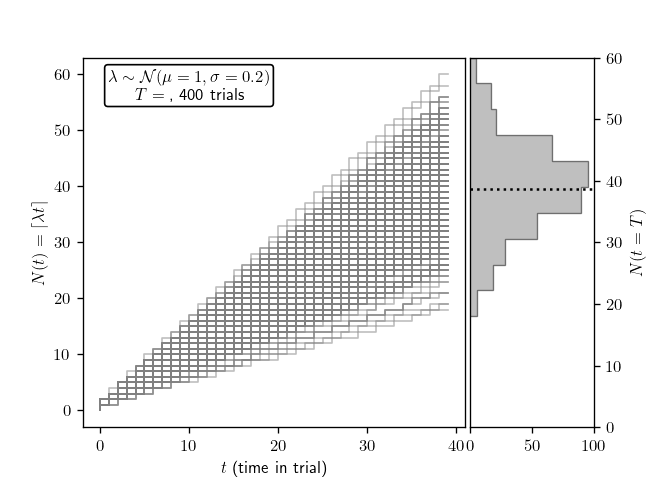
\includegraphics[scale=0.7]{nt_let}
            \caption{Example of a process of 400 trials. The left panel shows the state transitions for every
                    $\lambda$ sampled from the normal distribution in the textbox inset. At $T = 40$, the reinforced
                    states spread around the true value of $T$, so they aproximate a normal distribution with mean
                    $\mu \times t$ and standard deviation $\sigma \times t$ (right panel).}
    \end{figure}



\end{document}